% !TeX encoding = UTF-8
% !TeX program = pdflatex

\documentclass[11pt]{article}
\usepackage{graphicx}
\usepackage[T1]{fontenc}
\usepackage[utf8]{inputenc}
\usepackage[italian]{babel}
\usepackage{hyperref}

\title{\textbf{easyTravel} \\ \bigskip \large Laboratorio di Architetture Software e Sicurezza Informatica \\ Ingegneria Informatica e Automatica \\ Università degli Studi di Roma "La Sapienza"}
\author{Antonini Andrea 1707560\\Cariggi Gianmarco 1698481\\Costa Marco 1691388\\Pulicati Gianluca 1708686}
\date{\today}



\begin{document}
\maketitle

\pagebreak

\tableofcontents

\pagebreak

\section{Introduzione}

easyTravel è un sito che permette di confrontare prezzi e orari di voli, hotel e noleggio auto in molte
città italiane e le principali città europee, dando informazioni sul meteo della città di arrivo se la data è abbastanza vicina.


\section{Link github e tracking degli sprint}

Link github: \href{https://github.com/marcocosta96/easyTravel}{https://github.com/marcocosta96/easyTravel} \\
Link degli sprint: \href{https://docs.google.com/spreadsheets/d/14VnUUgNbMTW1_EG6KlEAEggAsf6aBKnaC1etXz5ji0I/edit#gid=12}{clicca qui} (TODO) %todo


\section{Istruzioni per l'avvio}

\begin{enumerate}
	\item Esegui \begin{verbatim}git clone https://github.com/marcocosta96/easyTravel\end{verbatim}
	\item Apri il terminale nel percorso del progetto ed esegui \begin{verbatim}bundle install\end{verbatim}
	\item Esegui \begin{verbatim}rails db:migrate && rails db:seed\end{verbatim} NOTA: per resettare il database, esegui il comando \begin{verbatim}rails db:reset\end{verbatim}
	\item Fai partire il server con il comando \begin{verbatim}rails server\end{verbatim}
	\item Clicca \href{localhost:3000}{localhost:3000} o \href{127.0.0.1:3000}{127.0.0.1:3000} oppure copiali sul vostro browser;
\end{enumerate}

Account di default:
\begin{itemize}
	\item Utente privato: username-> user@easytravel.test password-> usertest
	\item Utente aziendale: username-> company\_user@easytravel.test password-> companyusertest
	\item Admin: username-> admin@easytravel.test password-> admintest
\end{itemize}


\section{User stories}

\subsection{SIGNUP, LOGIN e LOGOUT}
\begin{enumerate}
	\item As an UNREGISTERED USER I want to SING UP USING EMAIL so that I can BECOME REGISTERED USER;
	\item As an UNREGISTERED USER I want to SING UP USING GOOGLE ACCOUNT so that I can BECOME REGISTERED USER;
	\item As an UNREGISTERED USER I want to SING UP USING EMAIL AND P. IVA so that I can BECOME REGISTERED COMPANY USER;
	\item As a REGISTERED USER I want to LOGIN USING EMAIL so that I can BECOME A LOGGED USER;
	\item As a REGISTERED USER I want to LOGIN USING GOOGLE ACCOUNT so that I can BECOME A LOGGED USER;
	\item As a REGISTERED USER I want to LOGIN USING EMAIL so that I can BECOME A LOGGED COMPANY USER;
	\item As a LOGGED USER I want to LOGOUT so that I can BECOME NON-LOGGED USER;
\end{enumerate}

\subsection{Gestione Users}
\begin{enumerate}
	\item As a REGISTERED USER I want to HAVE SETTINGS so that I can CHANGE MY EMAIL;
	\item As a REGISTERED USER I want to HAVE SETTINGS so that I can CHANGE MY PASSWORD;
	\item As a REGISTERED USER I want to HAVE SETTINGS so that I can RECOVER MY PASSWORD;
	\item As a REGISTERED USER I want to HAVE SETTINGS so that I can DELETE MY ACCOUNT;
	\item As a REGISTERED USER I want to HAVE SETTINGS so that I can SET AN AVATAR;
\end{enumerate}

\subsection{Unregistered User}
\begin{enumerate}
	\item As an UNREGISTERED USER I want to RESEARCH FOR FLIGHTS so that I can COMPARE SCHEDULES and PRICES;
	\item As an UNREGISTERED USER I want to SEE THE STATISTICS so that I can SEE THE GENERAL STATISTICS;
	\item As an UNREGISTERED USER I want to SEE THE WEATHER OF THE ARRIVAL CITY so that I CAN PLAN BETTER MY TRIP;
\end{enumerate}

\subsection{Registered User}
\begin{enumerate}
	\item As a REGISTERED USER I want to RESEARCH FOR FLIGHTS so that I can COMPARE SCHEDULES and PRICES;
	\item As a REGISTERED USER I want to SEE THE STATISTICS so that I can SEE THE GENERAL STATISTICS;
	\item As a REGISTERED USER I want to see the weather of the arrival city so that I can PLAN BETTER MY TRIP;
	\item As a REGISTERED USER I want to research for hotels in arrival city so that I can COMPARE PRICES;
	\item As a REGISTERED USER I want to SEE THE STATISTICS so that I can SEE GENERAL STATISTICS;
	\item As a REGISTERED USER I want to SEE THE STATISTICS so that I can SEE PERSONAL STATISTICS;
\end{enumerate}

\subsection{Company User}
\begin{enumerate}
	\item As a COMPANY USER I want to RESEARCH FOR FLIGHTS so that I can COMPARE SCHEDULES and PRICES;
	\item As a COMPANY USER I want to SEE THE STATISTICS so that I can SEE THE GENERAL STATISTICS;
	\item As a COMPANY USER I want to SEE THE WEATHER OF THE ARRIVAL CITY so that I can PLAN BETTER MY TRIP;
	\item As a COMPANY USER I want TO RESEARCH FOR HOTELS IN ARRIVAL CITY so that I can COMPARE PRICES;
	\item As a COMPANY USER I want to SEE THE STATISTICS so that I can SEE GENERAL STATISTICS;
	\item As a COMPANY USER I want to RESEARCH FOR CARS so that I can RENT A CAR;
\end{enumerate}

\subsection{Admin}
\begin{enumerate}
	\item As an ADMIN I want to HAVE AN USER LIST so that I can CHECK THE USERS OF THE WEBSITE;
	\item As an ADMIN I want to HAVE SPECIAL SETTINGS so that I can DELETE USERS;
\end{enumerate}

\pagebreak

\section{Schema DB}
\begin{figure}[!ht]
	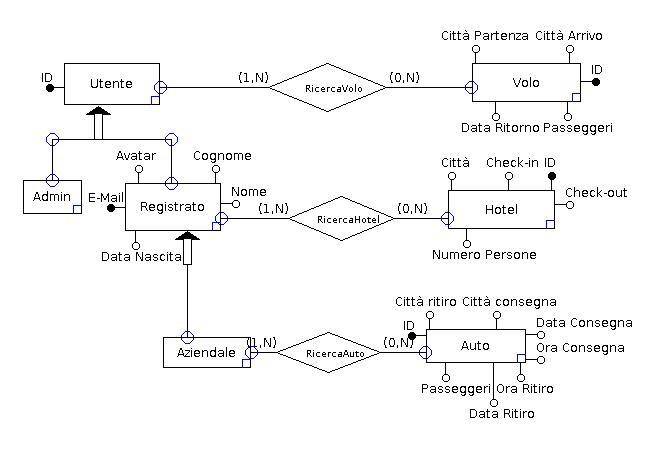
\includegraphics[width=1.2\textwidth]{progetto} % adjust width
	\caption{Schema ER realizzato mediante l'applicazione Java JDER v1.3}
	\label{fig:schemaer}
\end{figure}


\section{Struttura controllo degli accessi}
Sono previste due modalità di accesso:
\begin{itemize}
	\item Locale: L’utente inserisce le sue informazioni direttamente sul sito.
	\item OAuth: L’utente accede tramite Google e dà il consenso al trattamento dei propri dati, in questo modo è possibile compilare il form di registrazione e di accesso usando i dati del vostro account Google.
\end{itemize}

\subsection{Ruoli e diritti di accesso alle funzionalità disponibili}\label{roles}
I ruoli previsti all’interno dell’applicazione sono i seguenti:
\begin{itemize}
	\item Amministratore: ha accesso a tutte le impostazioni che riguardano il sito, può rimuovere commenti/utenti qualora lo ritenga necessario per evitare situazioni spiacevoli.
	\item Utente non registrato: può solamente fare ricerche di voli e consultare statistiche generali degli utenti che usano il sito.
	\item Utente registrato (Privato): oltre alle funzionalità concesse ad un utente non registrato, può fare ricerche sugli hotel, può salvare le ricerche effettuate, può impostare le città preferite e può consultare statistiche personali (come ore totali di viaggio, ecc...) e generali.
	\item Utente registrato (Aziendale): attivabile tramite apposito slider durante la registrazione, ha le stesse funzioni dell’utente privato, ma in più può fare ricerche sul noleggio auto. Può consultare solo le statistiche personali.
\end{itemize}


\section{Tecnologie utilizzate}
La web-app è basata sul paradigma \textbf{MVC (Model View Control)}.\\

\begin{large}\textbf{Linguaggi}\end{large}
\begin{itemize}
	\item Backend: Ruby on Rails;
	\item Frontend: HTML, Javascript, SAAS e CSS.
\end{itemize}

\begin{large}\textbf{Signin e signout}\\\end{large}
Per la registrazione e l'accesso ai servizi sono state usate le seguenti gemme:
\begin{itemize}
	\item Locale: gemma \href{https://github.com/plataformatec/devise}{\textbf{devise}};
	\item Google: gemma \href{https://github.com/zquestz/omniauth-google-oauth2}{\textbf{omniauth-google-oauth2}}.
\end{itemize}

\begin{large}\textbf{Informazioni meteo}\end{large}\\ 
Attraverso la gemma \href{https://github.com/coderhs/ruby_open_weather_map}{\textbf{open-weather}}, possiamo cercare informazioni sul meteo per le città selezionate se è disponibile per il giorno della partenza.
\\\\\\
\begin{large}\textbf{Informazioni voli}\end{large}\\
Per le informazioni sui voli, utilizziamo le \textbf{API REST} del servizio \href{https://aviation-edge.com/}{Aviation Edge}. Tramite questo sito è possibile consultare tutte le informazioni riguardanti gli aeroporti delle città selezionate e gli orari dei voli. Inoltre tramite apposito pulsante è possibile fare redirect al sito \href{https://www.skyscanner.it}{Skyscanner} con cui poter confrontare i prezzi e procedere all'acquisto tramite il loro portale.
\\\\
\begin{large}\textbf{Informazioni hotel e autonoleggio}\end{large}\\
Per quanto riguarda questi due servizi, è implementato un redirect al sito \href{https://www.skyscanner.it}{Skyscanner} in cui poter confrontare prezzi e procedere all'acquisto, come accade per i voli.
\\\\
\begin{large}\textbf{Ruoli}\end{large}\\
Per la distinzione dei vari servizi dedicati a specifici ruoli, abbiamo usato la gemma \href{https://github.com/RolifyCommunity/rolify}{\textbf{rolify}}. Le funzionalità assegnate ad ognuno di loro sono state illustrate nella precedente sezione \ref{roles}.
\\\\
\begin{large}\textbf{Realizzazione del frontend}\end{large}\\
Il front-end è stato realizzato usando il framework \href{https://github.com/Dogfalo/materialize}{\textbf{Materialize}}. Esso si basa principalmente sul linguaggio CSS e sul link indicato è disponibile la documentazione completa.


\section{Piano dei Test}

\pagebreak


\section{Mockup}
\begin{figure}[!ht]
	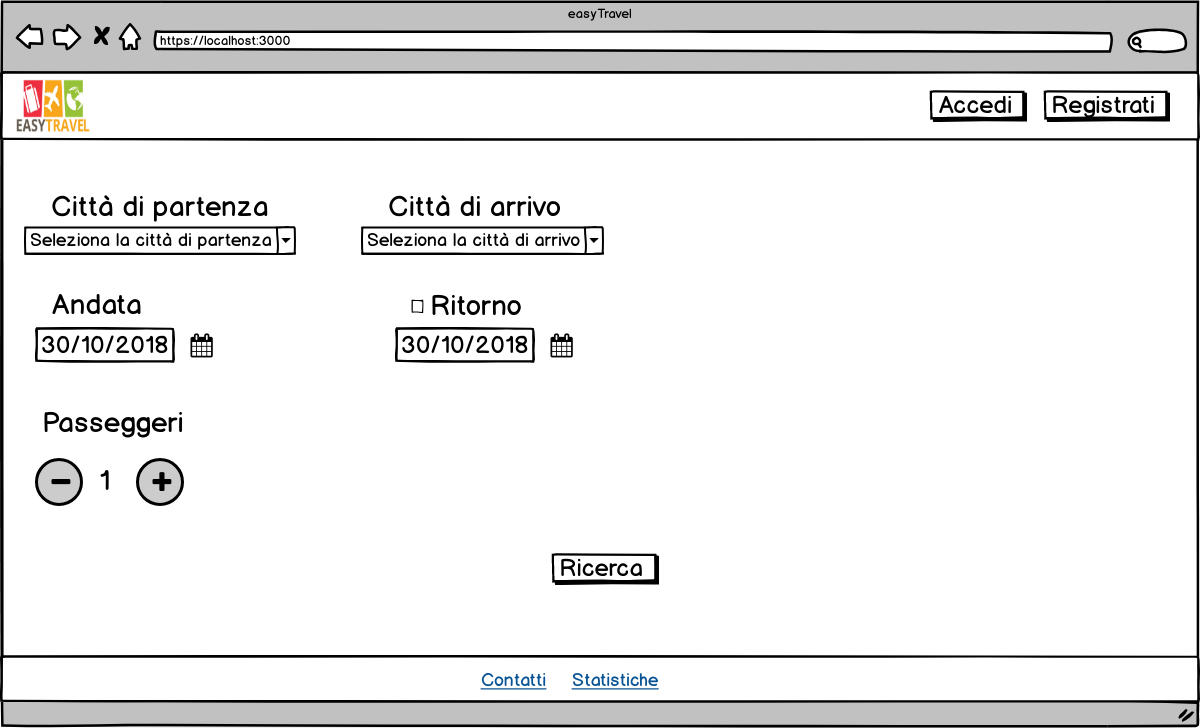
\includegraphics[width=1\textwidth]{./Mockup/Home-non-registrato} % adjust width
	\caption{Schermata home quando non si è registrati}
	\label{fig:homenotreg}
\end{figure}

\begin{figure}[!ht]
	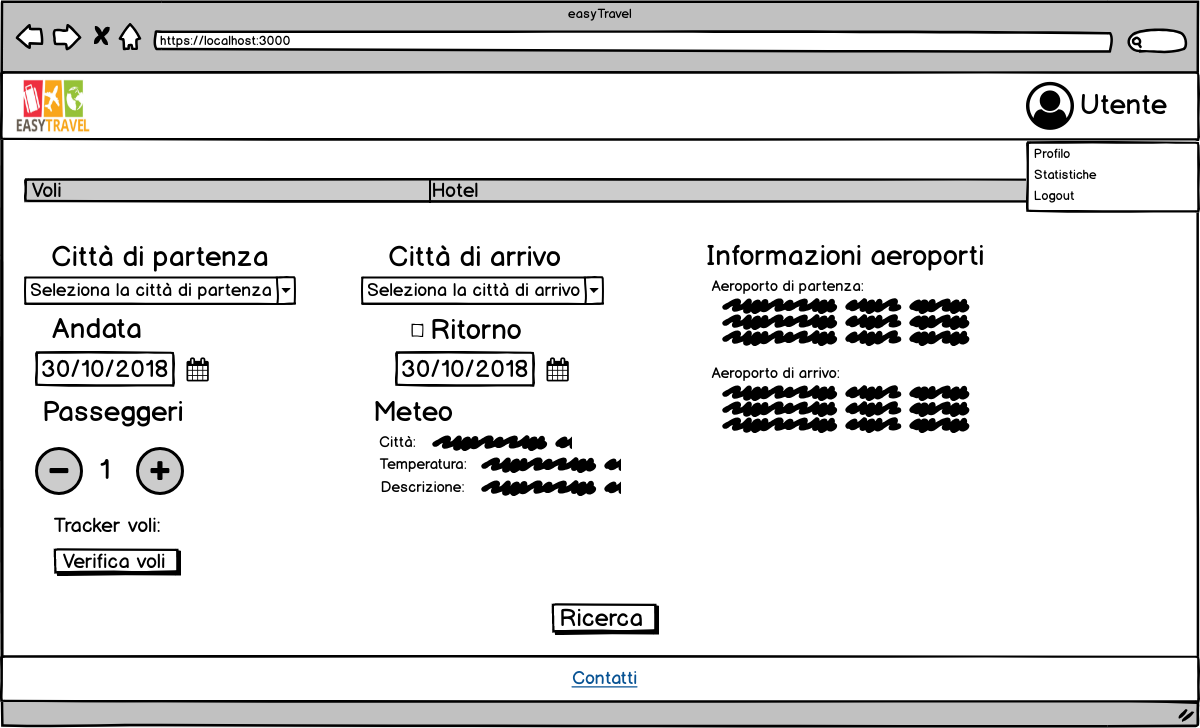
\includegraphics[width=1\textwidth]{./Mockup/Voli-user} % adjust width
	\caption{Schermata home quando si è registrati come utente Privato}
	\label{fig:homeuser}
\end{figure}

\begin{figure}[!ht]
	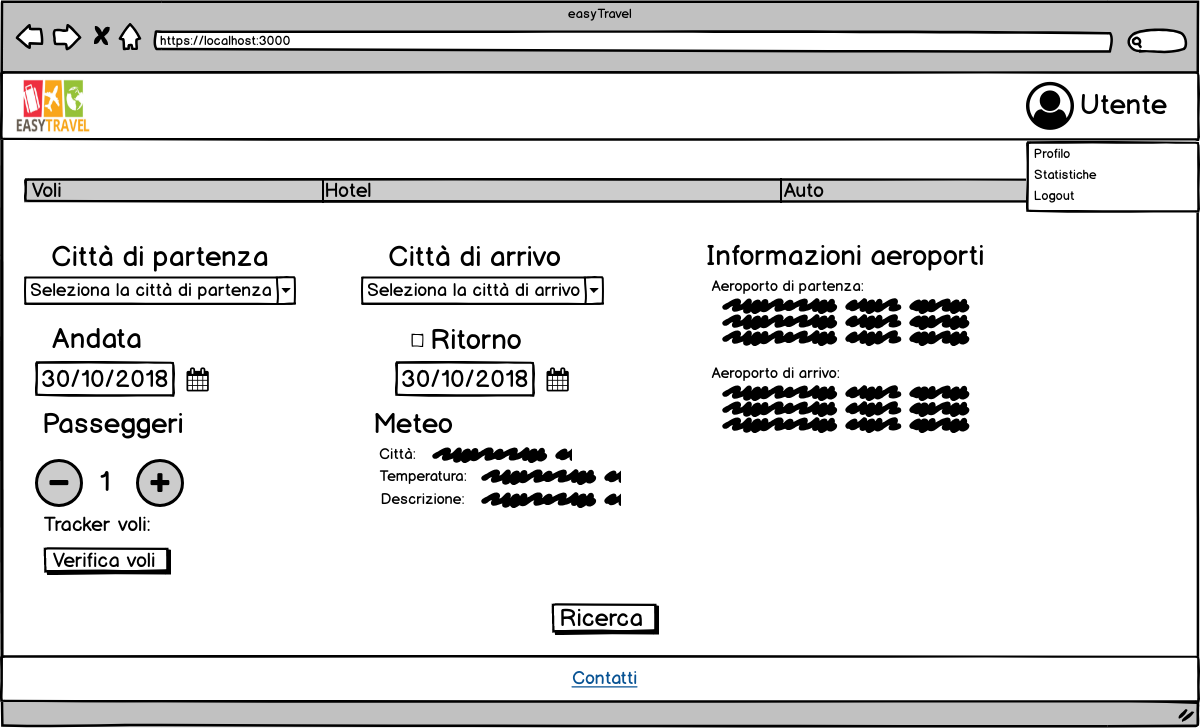
\includegraphics[width=1\textwidth]{./Mockup/Voli-aziendale-admin} % adjust width
	\caption{Schermata home quando si è registrati come utente Aziendale o Admin}
	\label{fig:homeaziendaleadmin}
\end{figure}

\begin{figure}[!ht]
	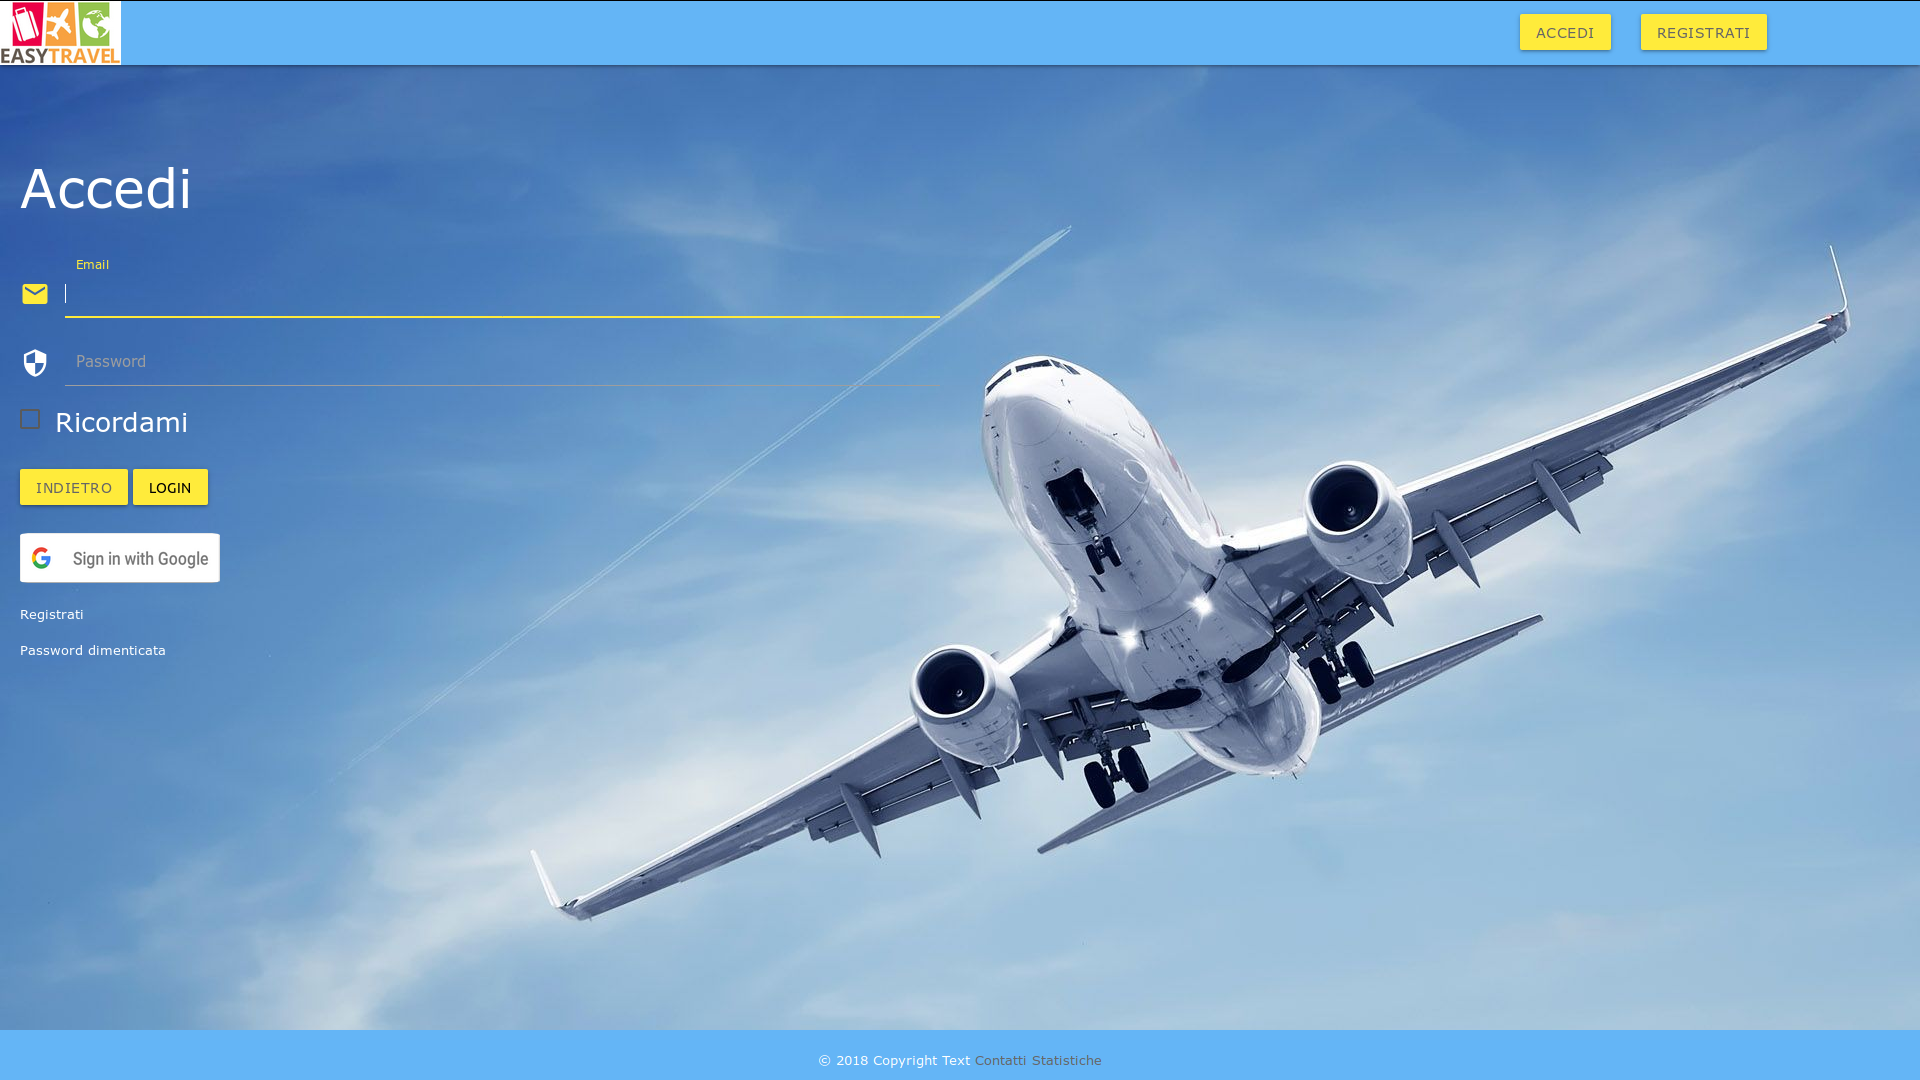
\includegraphics[width=1\textwidth]{./Mockup/Accesso} % adjust width
	\caption{Schermata per l'accesso}
	\label{fig:accesso}
\end{figure}

\begin{figure}[!ht]
	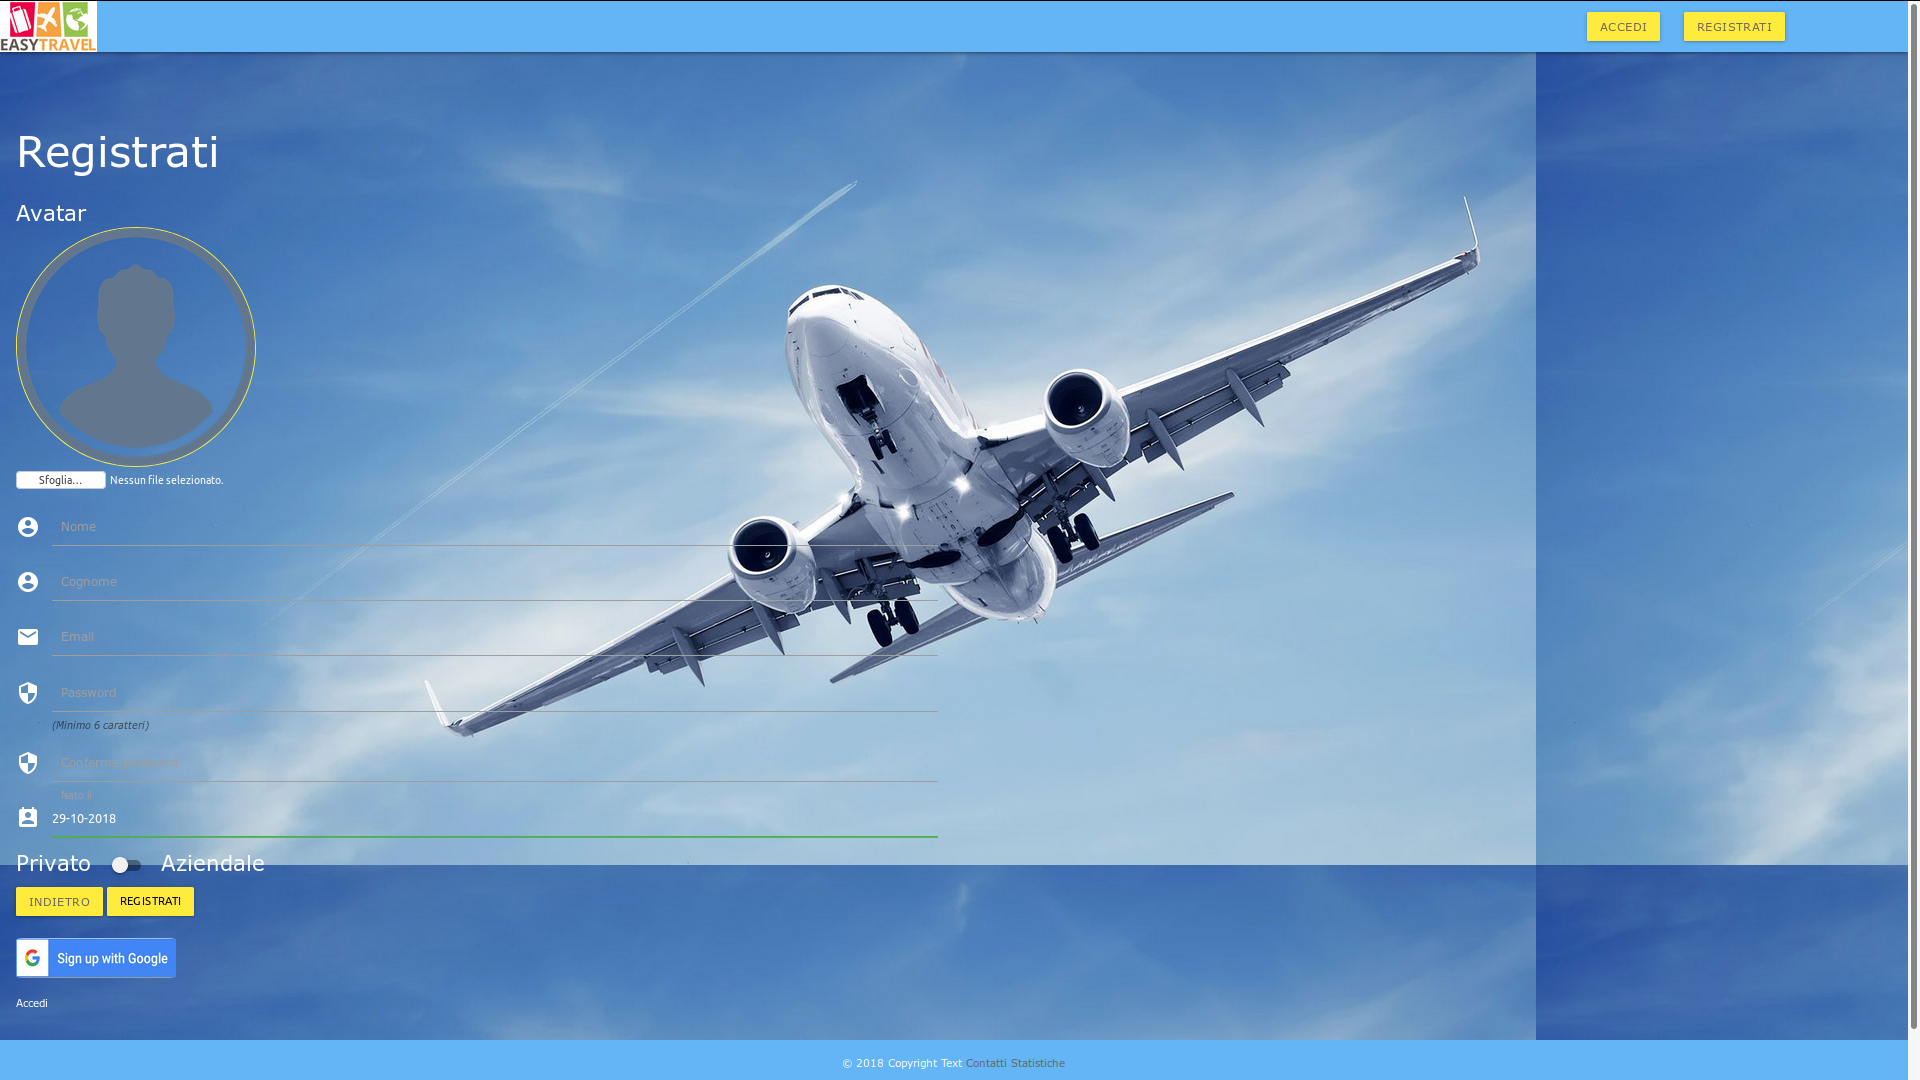
\includegraphics[width=1\textwidth]{./Mockup/Registrazione} % adjust width
	\caption{Schermata per la registrazione}
	\label{fig:registrazione}
\end{figure}

\begin{figure}[!ht]
	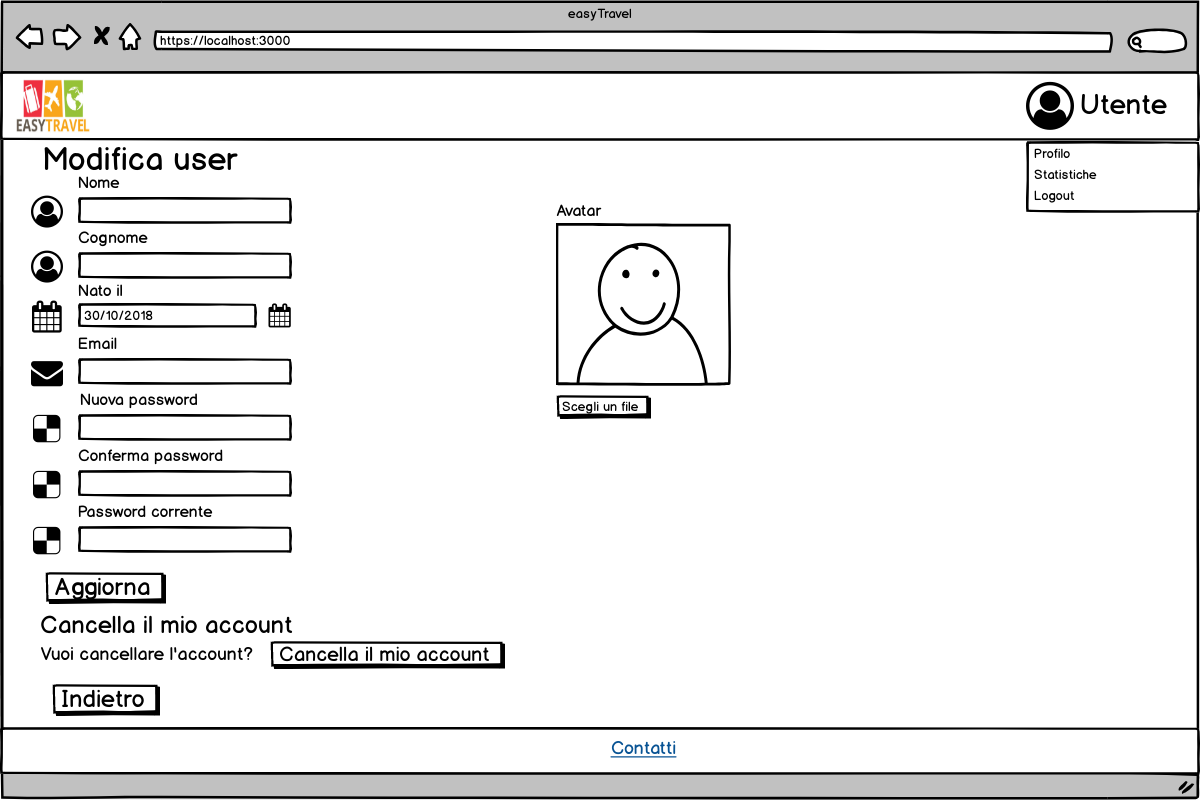
\includegraphics[width=1\textwidth]{./Mockup/Profilo-user-aziendale} % adjust width
	\caption{Schermata con le informazioni personali}
	\label{fig:profiloutente}
\end{figure}

\begin{figure}[!ht]
	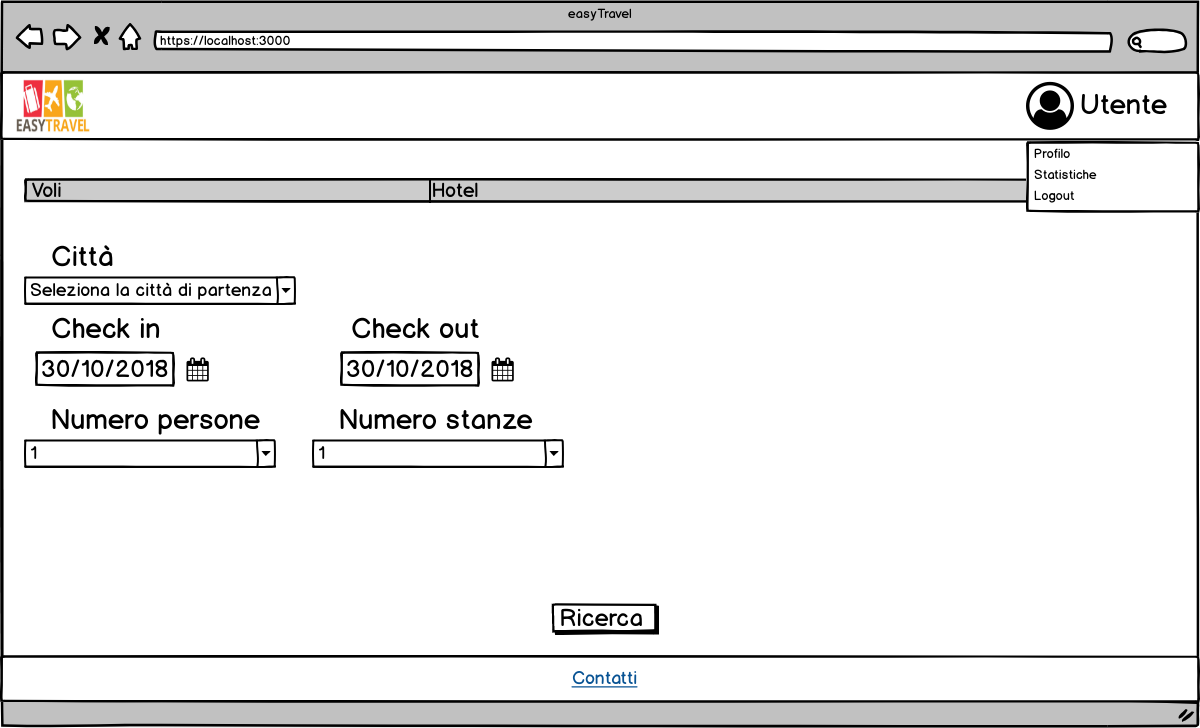
\includegraphics[width=1\textwidth]{./Mockup/Hotel-user} % adjust width
	\caption{Schermata per la scelta dell'hotel quando si è registrati come utente Privato}
	\label{fig:hoteluser}
\end{figure}

\begin{figure}[!ht]
	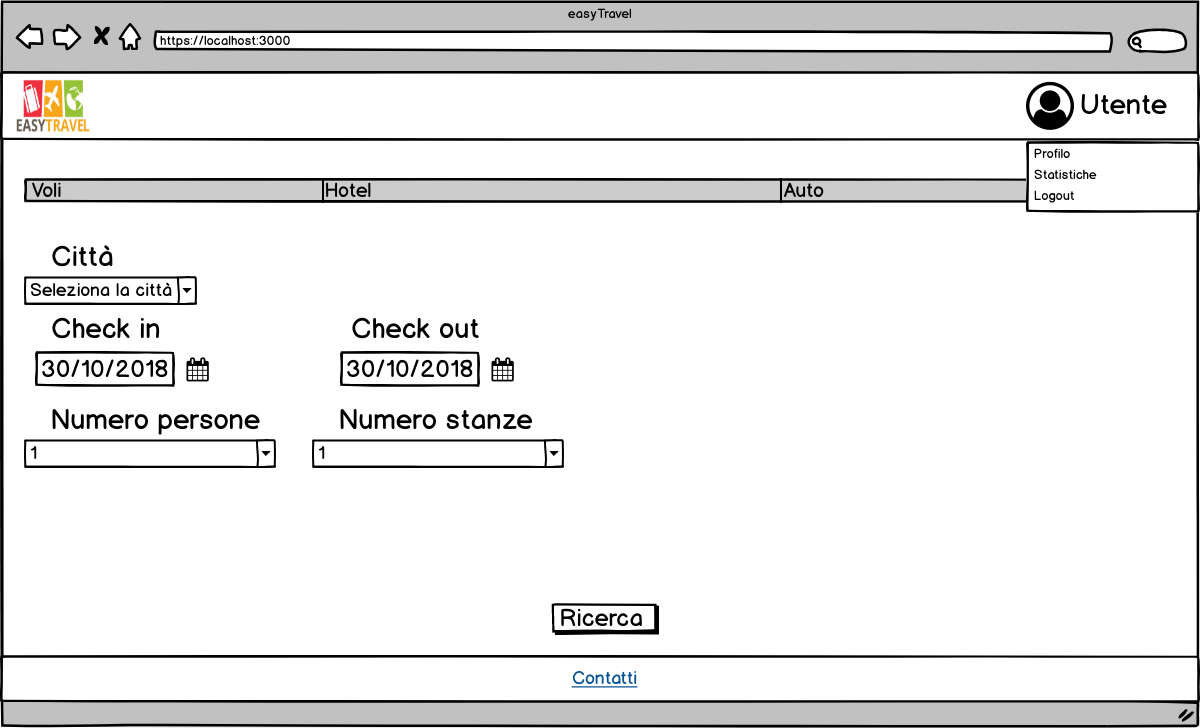
\includegraphics[width=1\textwidth]{./Mockup/Hotel-aziendale-admin} % adjust width
	\caption{Schermata per la scelta dell'hotel quando si è registrati come utente Aziendale o Admin}
	\label{fig:hotelaziendaleadmin}
\end{figure}

\begin{figure}[!ht]
	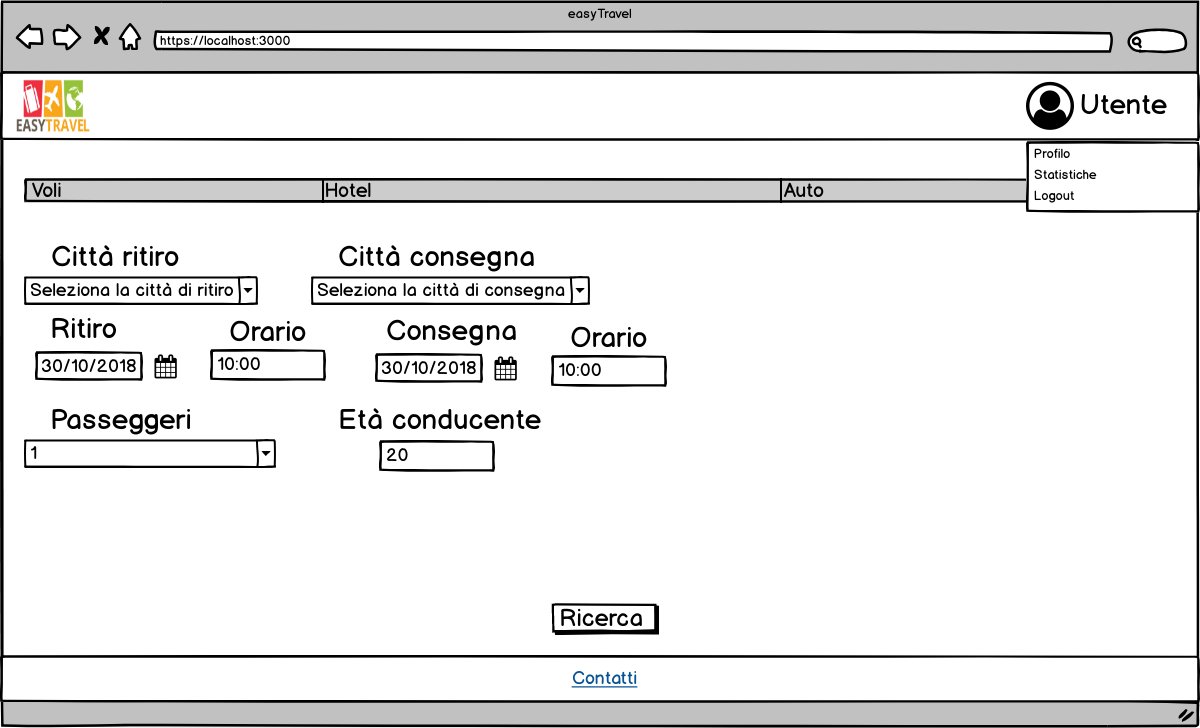
\includegraphics[width=1\textwidth]{./Mockup/Auto-aziendale-admin} % adjust width
	\caption{Schermata per la scelta del noleggio auto quando si è registrati come utente Aziendale o Admin}
	\label{fig:autoaziendaleadmin}
\end{figure}

\begin{figure}[!ht]
	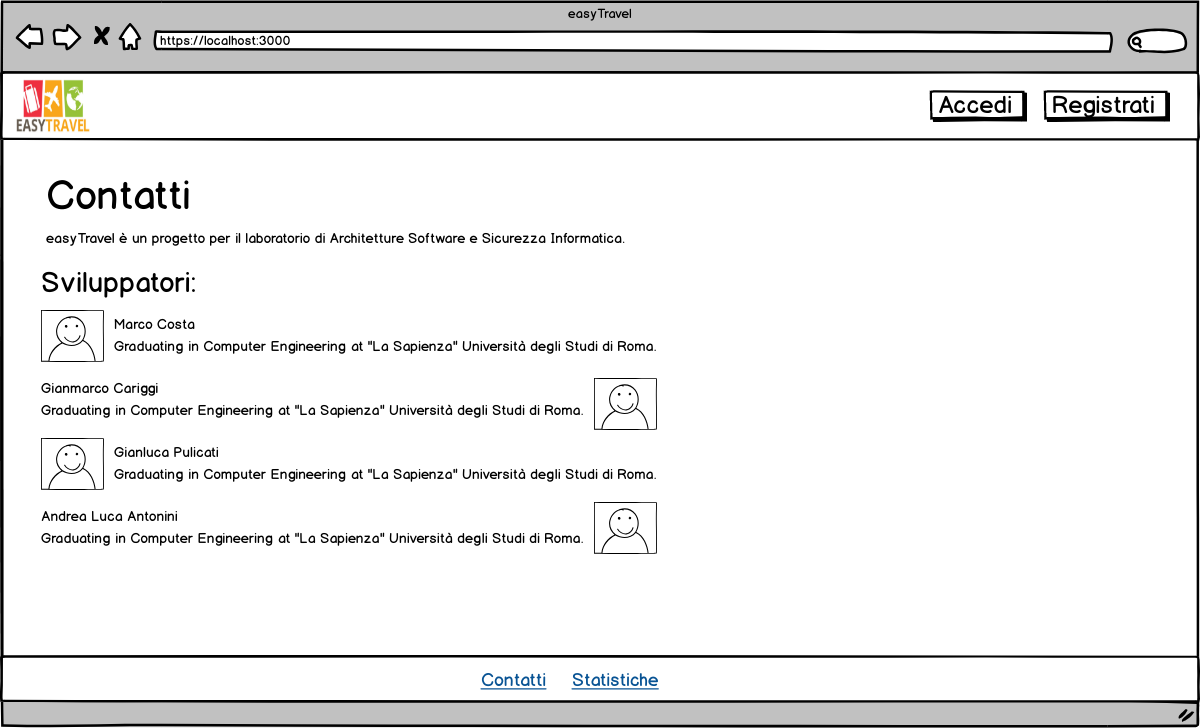
\includegraphics[width=1\textwidth]{./Mockup/Contatti-non-registrato} % adjust width
	\caption{Schermata con le informazioni dello staff}
	\label{fig:contattinonreg}
\end{figure}

\begin{figure}[!ht]
	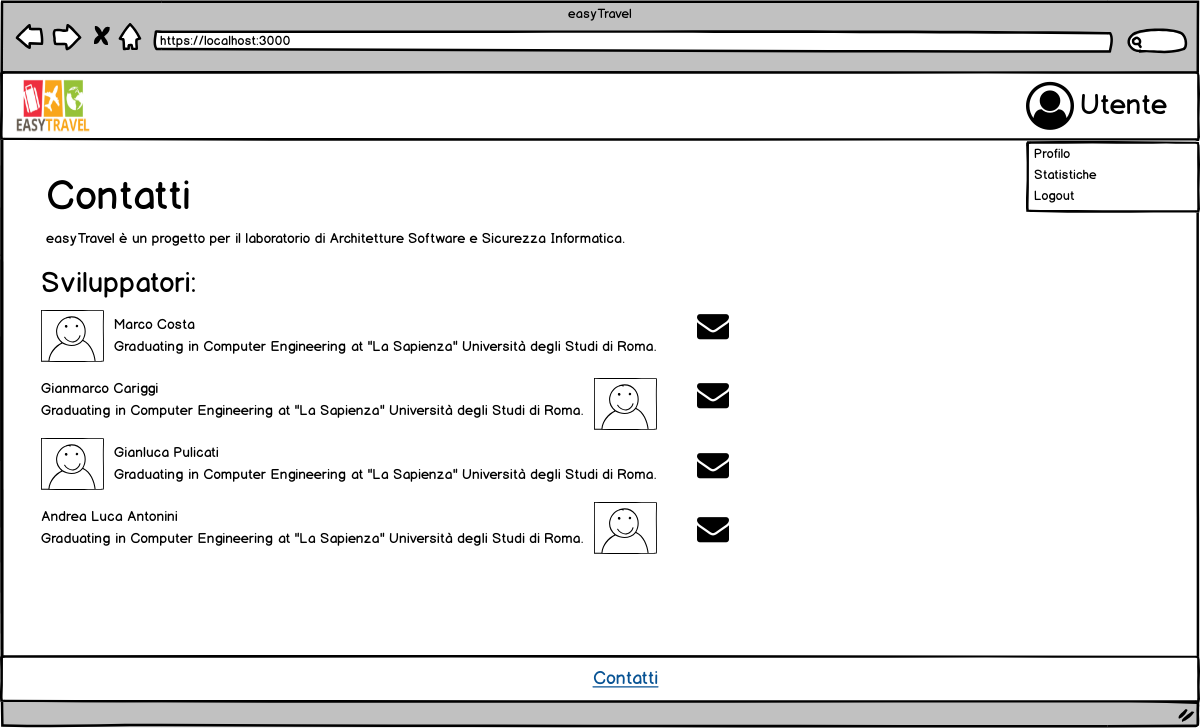
\includegraphics[width=1\textwidth]{./Mockup/Contatti-registrato} % adjust width
	\caption{Schermata con i contatti e le informazioni dello staff}
	\label{fig:contattireg}
\end{figure}

\begin{figure}[!ht]
	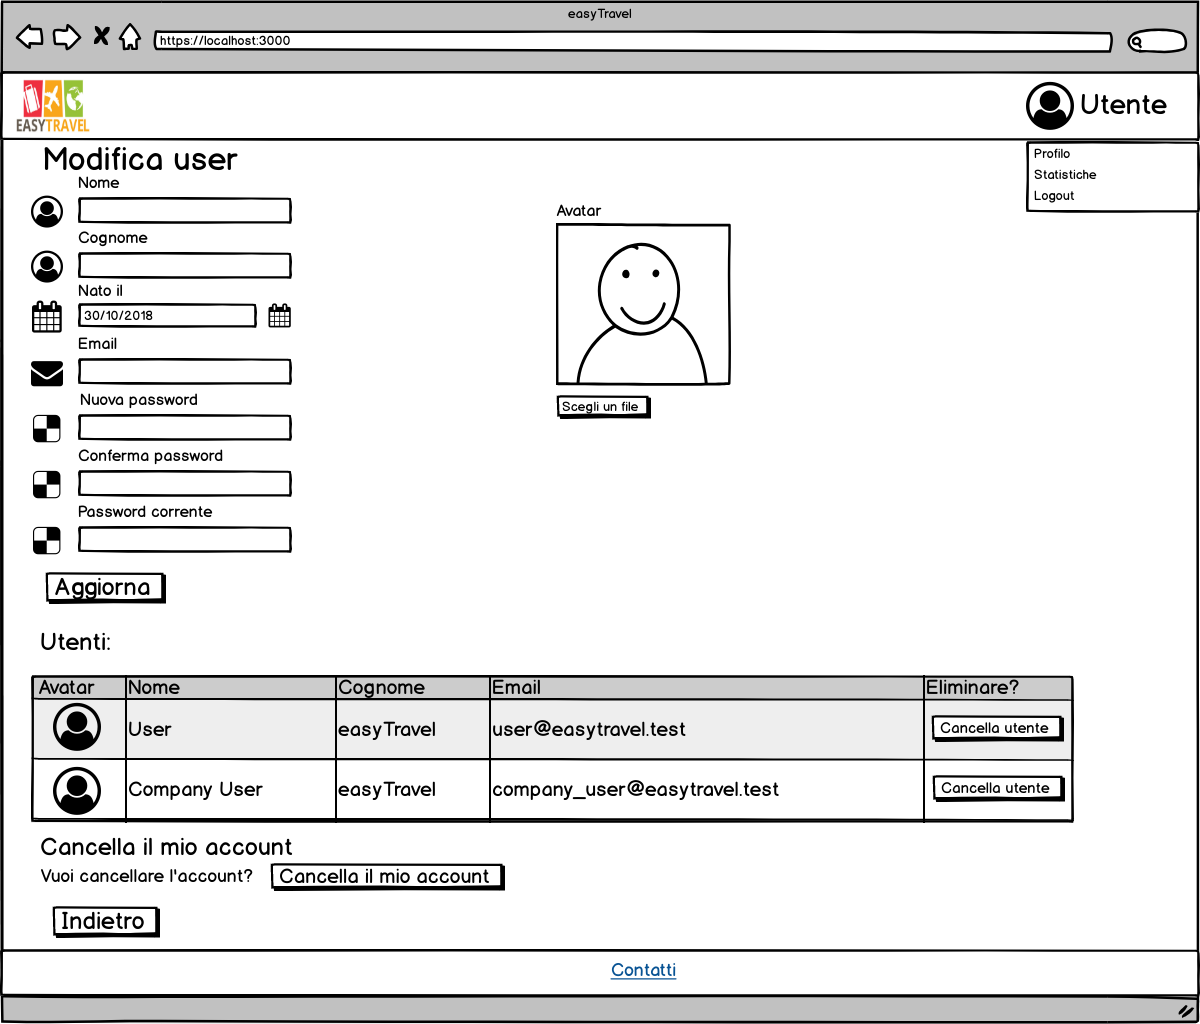
\includegraphics[width=1\textwidth]{./Mockup/Profilo-admin} % adjust width
	\caption{Schermata con la dashboard a disposizione per l'admin}
	\label{fig:profiloadmin}
\end{figure}

\begin{figure}[!ht]
	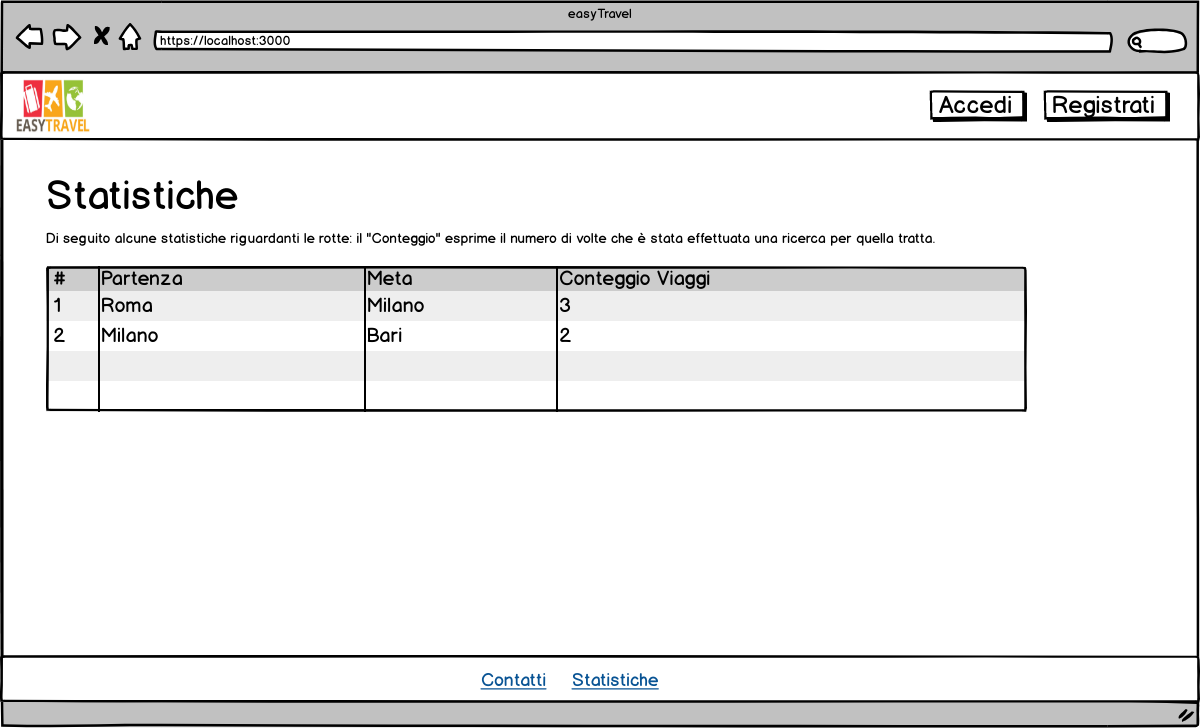
\includegraphics[width=1\textwidth]{./Mockup/Statistiche-non-registrato} % adjust width
	\caption{Schermata con le statistiche generali per un utente non registrato}
	\label{fig:statistichenonreg}
\end{figure}

\begin{figure}[!ht]
	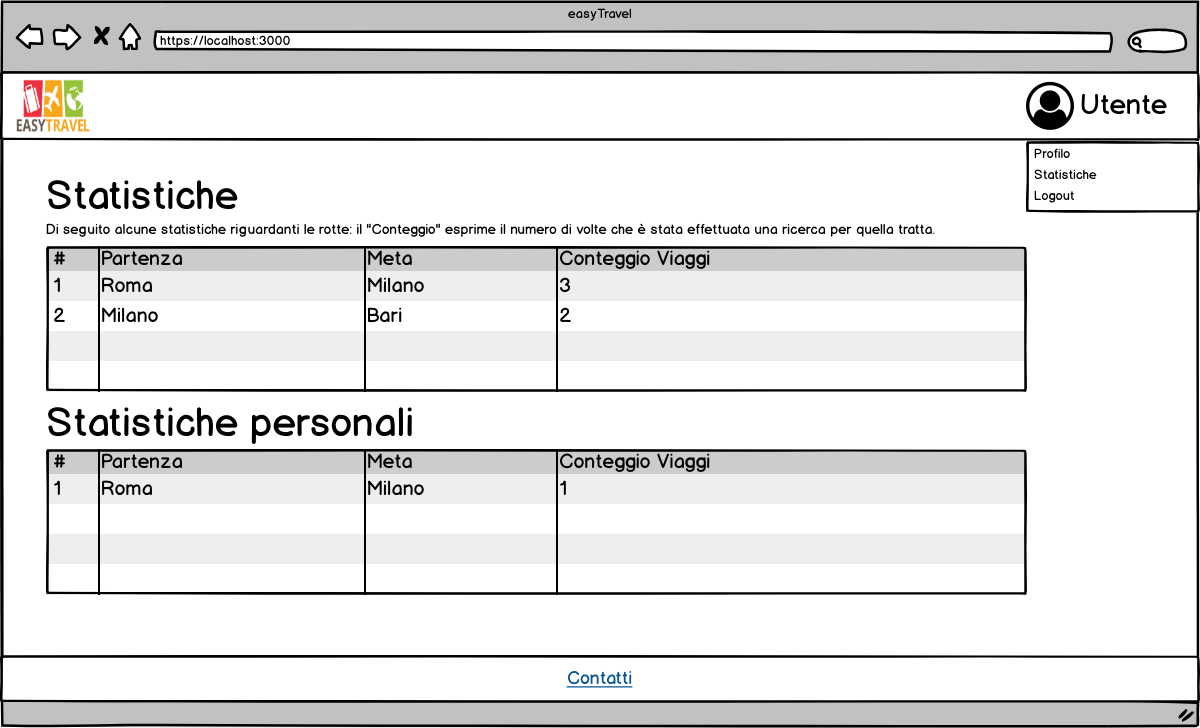
\includegraphics[width=1\textwidth]{./Mockup/Statistiche-user-admin} % adjust width
	\caption{Schermata con le statistiche generali per un utente registrato o per un admin}
	\label{fig:statisticheuseradmin}
\end{figure}

\begin{figure}[!ht]
	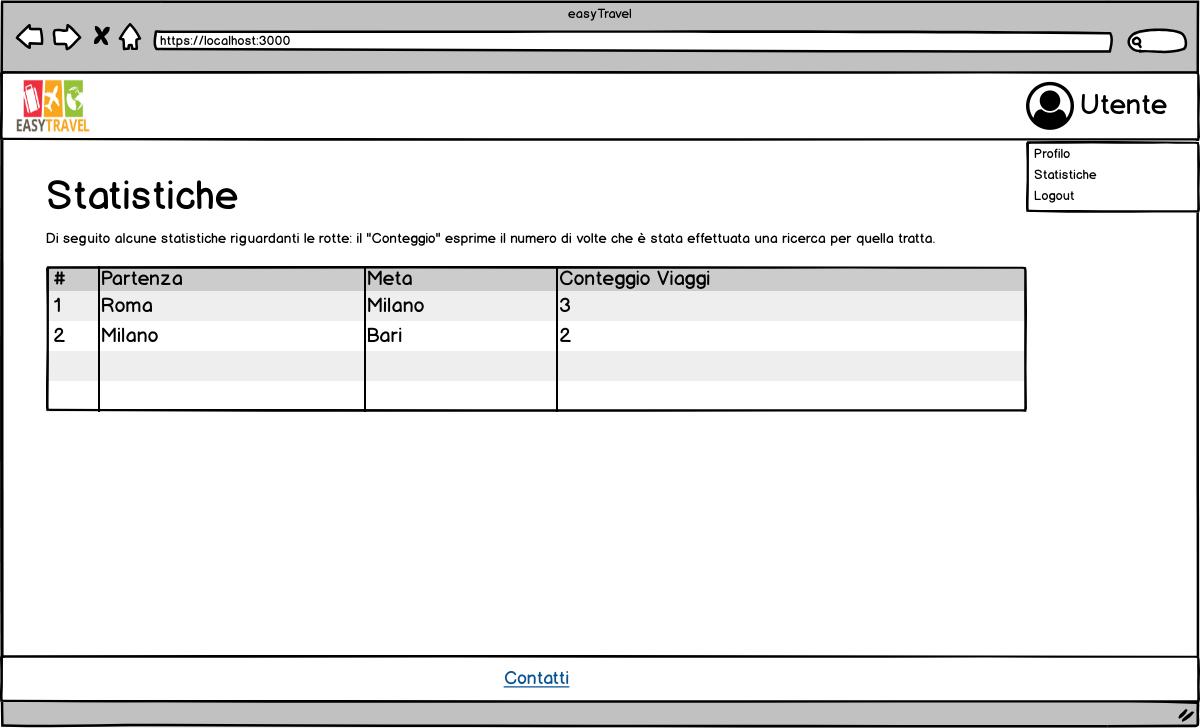
\includegraphics[width=1\textwidth]{./Mockup/Statistiche-aziendale} % adjust width
	\caption{Schermata con le statistiche generali per un utente aziendale}
	\label{fig:statisticheaziendale}
\end{figure}


\end{document}
